\section{Central Posterior Interval}

A central posterior interval or credible interval of confidence level $\alpha$ is an interval $[a, b]$ such that:

$$ P(\mu | \bar{x} \in [a, b]) = \alpha $$

Credible intervals are not unique for a given posterior distribution.
\textbf{High Density Interval} (HDI) is the smallest credible interval with confidence level $\alpha$.
In other words, high density interval of confidence level $\alpha$ is $[a, b]$ such that:

\[ a, b = \argmin_{a, b \, : \, P(\mu | \bar{x} \in [a, b]) = \alpha} b - a \]

Since our conjugate prior is normal, the high density interval will be centered about the mean of the posterior distribution.
Hence, if the posterior distribution is $\mu | \bar{x} \sim N(u', v')$ with CDF $F$, the high density interval of confidence level $\alpha$ will be $[u' - c, u' + c]$ such that:

\begin{align*}
&P(\mu |\bar{x} \in [u' - c, u' + c]) = \alpha \\
&\Rightarrow F(u' + c) - F(u' - c) = \alpha \\
&\Rightarrow 1 - 2F(u' - c) = \alpha \\
&\Rightarrow F(u' - c) = \frac{1 - \alpha}{2} \\
&\Rightarrow \Phi(\frac{(u' - c) - u'}{\sqrt{v'}}) = \frac{1 - \alpha}{2} \\
&\Rightarrow \Phi(-\frac{c}{\sqrt{v'}}) = \frac{1 - \alpha}{2} \\
&\Rightarrow -\frac{c}{\sqrt{v'}} = \Phi^{-1}\left(\frac{1 - \alpha}{2}\right) \\
&\Rightarrow c = -\sqrt{v'} \cdot \Phi^{-1}\left(\frac{1 - \alpha}{2}\right)
\end{align*}

\noindent where $\Phi$ is the CDF of the standard normal distribution.

Refer to \autoref{fig:hdi} for 95\% posterior HDI with $n = 10$.

\begin{figure}
    \centering
    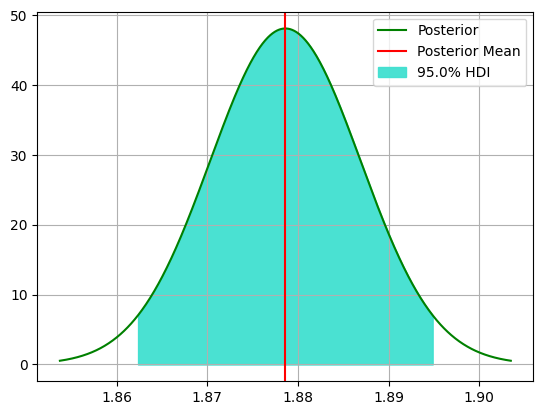
\includegraphics[width=.6\linewidth]{images/hdi.png}
    \caption{95\% confidence posterior HDI}
    \label{fig:hdi}
\end{figure}
